%% -*- mode: LaTeX -*-
%%

%%%%%%%%%%%%%%%%%%%%%%%%%%%%%%%%%%%%%%%%%%%%%%%%%%%%%%%%%%%%%%%%%%%%%%%%%%%%%%%

\section{Background}
\label{sec:background}

\begin{figure}
  \centering
  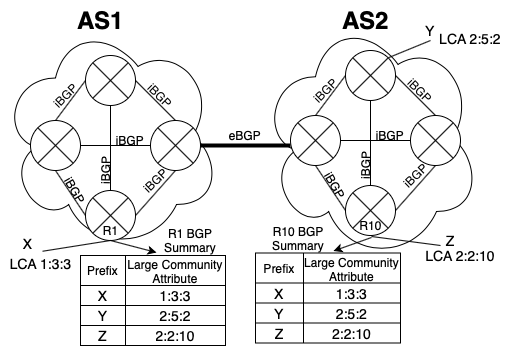
\includegraphics[width=0.9\columnwidth]{BGPFig}
  \caption{BGP Advertisement with Large Community Attribute}
  \label{fig:example1}
\end{figure}
In our work we use BGP and Segment Routing to create a novel service specific Inter- and intra-domain
routing framework. The combination of BGP working at the control plane and Segment Routing working at
the data plane gives the ability to have more control on the treatment of service specific traffic across ASes.

BGP~\cite{BGPPolicy} is the defacto exterior gateway protocol designed to exchange routing and 
reachability information between ASes. Internal BGP (iBGP), and external BGP (eBGP) are two forms of 
BGP. Given away by there respective names they either operate within (internal) the AS, or between (external)
 ASes. ASes will peer with neighboring ASes to exchange routing information and policy. Thus an eBGP connection
between ASes at the TCP level is establish to exchange advertised prefixes. From there iBGP connections
within the AS at the TCP level are established with surrounding routers to propagate the prefixes acquired
from the neighboring AS. As you can see this works with all connected ASes, therefore an AS can know
of an AS two or three neighbors away without a direct connection to it. 

For the control plane, we use BGP's Large Community Attribute~\cite{largeBGP}  to advertise the service
specific routes from the service provider to its adjacent and non-adjacent ASes. BGP already contains 
multiple attributes that help define the prefix that's being advertised. Large community attribute is already
allowed to be advertised with the BGP prefix, thus there is no need to add or change BGP in any away. Our
approach revolves around using already defined attributes in a new way. The large community attribute 
consists of three 4-octet values. The only required step is for a network operator to configure these
values. The first octet defines the AS number of the advertising AS, while the remaining two octets 
define the function and parameters associated with the community. Ideally ASes will receive the prefix
advertisements and associate the prefix with a specific service for the traffic destined to this prefix. 
\textbf{Figure~\ref{fig:example1}} is an example illustration of BGP Advertisements.

Internet Protocol version 6 (IPv6)~\cite{ipv6} is the most recent version of the internet protocol. IPv6 
in the near future is intended to replace IPv4. IPv6 is the preferred method for segment routing. IPv6
contains an extension header that was designed to offer flexibility by augmenting the IPv6 header with 
a set of instructions. There are six different types of extension headers, but the most important for our
purposes is the "routing header." The routing header is used by an IPv6 source to list one or more
intermediate nodes to be "visited" on the way to a packet's destination. As you will read about this in the 
next paragraph this sounds a lot like segment routing. Thus IPv6 is an ideal candidate because of its 
segment routing header capabilities and because it's the newest version of IP.

\begin{figure}
  \centering
  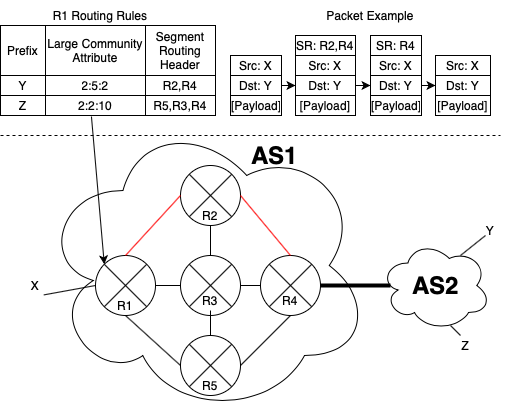
\includegraphics[width=0.9\columnwidth]{SRFIG}
  \caption{Segment Routed traffic based on BGP large community attribute}
  \label{fig:example2}
\end{figure}
Segment Routing~\cite{SRINFO} involves a packet being steered through a network topology. A segment can represent
any instruction, topological or service based. But for our purposes segments represent IPv6 addresses
within an AS. When a host is ready to send traffic through a network, the router will attach a routing header
to the IPv6 packet. The routing header will contain a list of IPv6 addresses (segments) that guide the packet
through the network before it reaches its destination. As stated in the previous paragraph, segment routing 
can be directly applied to the IPv6 architecture. \textbf{Figure~\ref{fig:example2}} is an example illustration 
of Segment Routing involving BGP large community attribute.

%%%%%%%%%%%%%%%%%%%%%%%%%%%%%%%%%%%%%%%%%%%%%%%%%%%%%%%%%%%%%%%%%%%%%%%%%%%%%%%

%% End of file.






